\section{About the IR Camera}
\label{sec:icam}
The IR Camera, an Onca-MWIR-InSb from Xenics, is the main device used in this dissertation and its function is to give an "image" of the analyzed object's temperature field. Its 2D array of sensors reads the incident IR radiation. Its signal is then converted to temperature in the camera's software. The user will end up with a bi-dimensional field of temperatures with a +/- 0.5ºC precision. This camera can be seen in Figure \ref{fig:onca}.

\begin{figure}[h!]
\centering
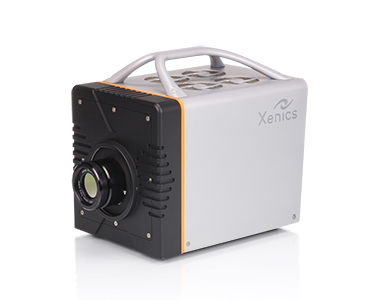
\includegraphics[width=0.6\linewidth]{Figures/2.Chapter/onca.png}
\caption{Xenics' Onca-MWIR-InSb}
\source{http://www.xenics.com/en/onca-mwir-insb}
\label{fig:onca}
\end{figure}

\subsection{Camera properties}

\par The relevant properties of the Onca-MWIR-InSb can be seen in Table \ref{tab:camprop}.

\begin{table}[h]
\centering
\caption{Camera Properties}
\label{tab:camprop}
\begin{tabular}{lclclc}
\toprule
\multicolumn{2}{c}{Camera Characteristics} & \multicolumn{2}{c}{Optical System} & \multicolumn{2}{c}{Image Characteristics} \\
\cmidrule[0.4pt](r{0.125em}){1-2}%
\cmidrule[0.4pt](r{0.125em}){3-4}%
\cmidrule[0.4pt](r{0.125em}){5-6}%
Sensor                 & InSb (MWIR)       & Focal lens          & 13 mm        & Video Rate         & 60Hz                 \\
Spectral Sensibility   & 3.5-5 $\mu m$     & Optics Material     & Germanium    & Max framerate      & 3000 fps             \\
Spatial Resolution     & $320 \times 256$  &  -                  & -            & Min pixels (ROI)   & $15 \times 5$        \\
Thermal Sensibility    & \textless17mk     &   -                 &   -          & Exposition         & \textgreater 1 $\mu s$  \\ \bottomrule
\end{tabular}
\end{table}


\subsection{The Software}

\par This camera has its own specific software, Xeneth, which will be very important throughout this work. It's relevant to explain its functioning, which will be referenced various time in this dissertation.

\subsubsection{Selecting a Calibration Pack}

\par When the program is executed a menu will appear. In this menu it's possible to select not only the used camera (there is also an option to select a virtual camera, used to play previously recorded videos) but also to select a calibration pack as it is shown in Figure \ref{fig:consetup}.
\begin{figure}[h]
\centering
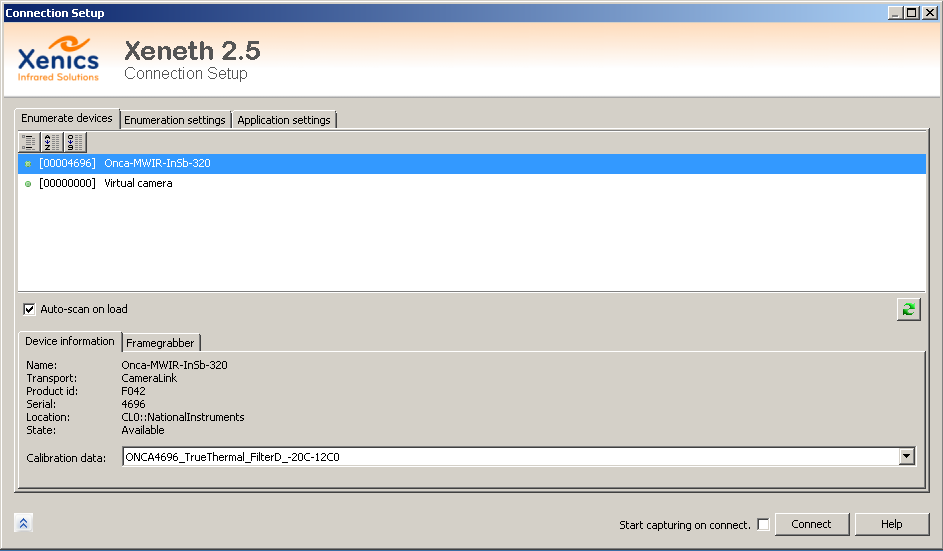
\includegraphics[width=0.7\linewidth]{Figures/3.Chapter/xeneth1.png}
\caption{Xeneth: Connection Setup Menu}
\label{fig:consetup}
\end{figure}
\par In the Calibration data drop menu are available several calibration packs. The main packs are:
\begin{itemize}
\item TRUE NUC: This pack is the one chosen if one wants to get data without temperature conversion. It presents results in ADU (received signal intensity) and it's adaptable to any integration time
\item TRUE THERMAL: This pack comes with a factory made calibration, so the results are presented in Celsius. This is used if the user just pretends a low thermal resolution measure or a qualitative result. It measures temperatures from -20 to 120ºC in any integration time.
\item User Calibration Packs: The user may want to create his own pack adapted to his own temperature interval, to use in a more precise application.
\end{itemize}

\subsubsection{Main Window}
\label{software}
\par After choosing the right calibration for the desired application and before starting the measurements, one should adjust several parameters in the main software window. The displayed panels can be shown in Figure \ref{fig:xeneth2}. There is a panel for the Camera Image, where one can see the thermal image and select an area or dot to take its read value and other statistics; a User Interaction Panel, where one can change settings, view and set the selection properties, record and save videos and choose image filters; a panel that shows the plotted measured data. In the right side we can also see a colour bar. This bar is adjustable so that we can adapt the colour gradient to the desired temperature interval to better observe the phenomena. \\
\begin{figure}[h]
\centering
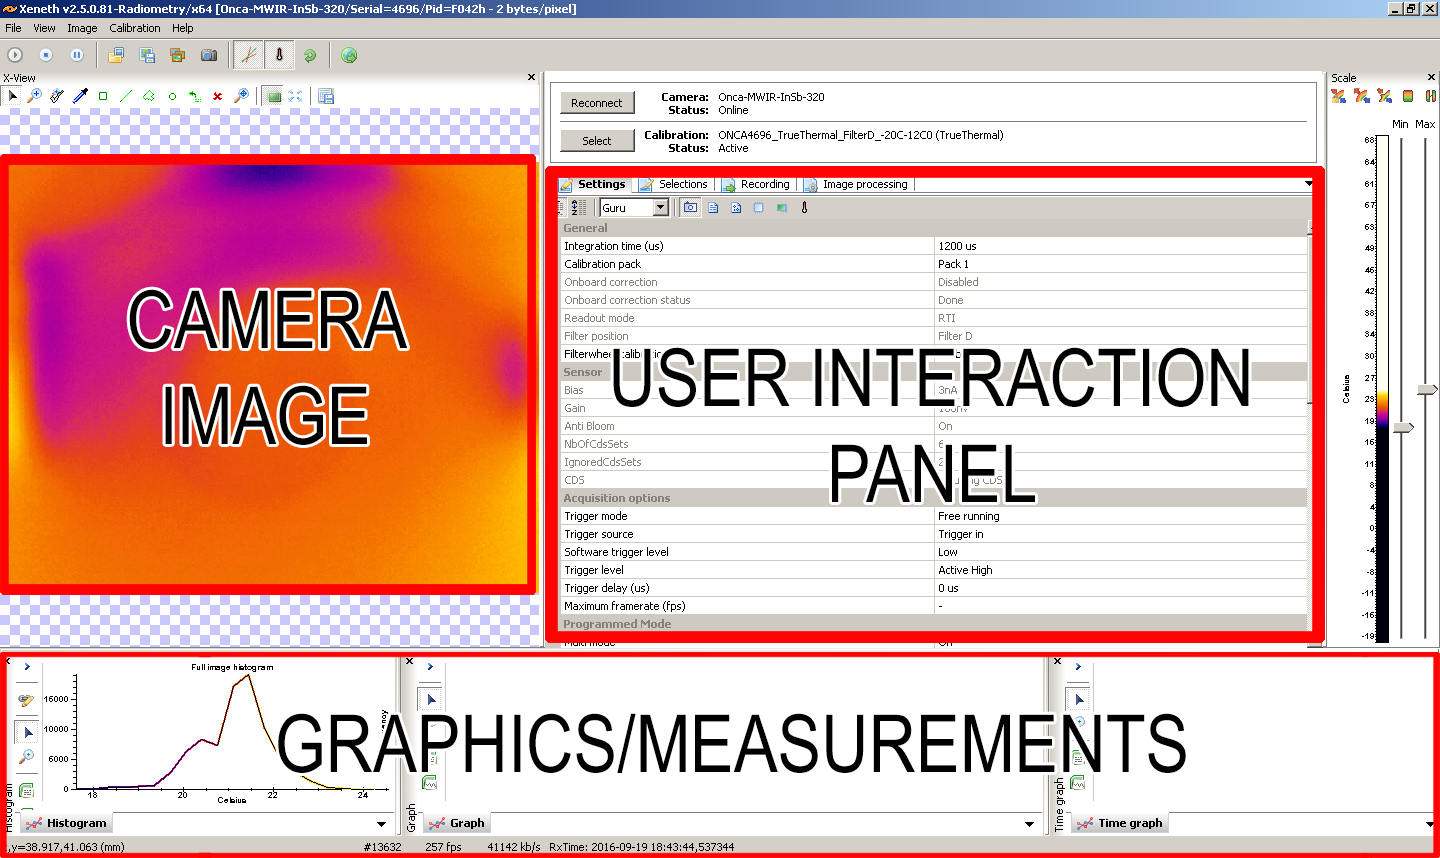
\includegraphics[width=0.7\linewidth]{Figures/3.Chapter/xeneth2.png}
\caption{Xeneth: Main Window Scheme}
\label{fig:xeneth2}
\end{figure}
\par Before starting there are some important settings to review to assure the best image possible. These parameters can be altered in the User Interaction Panel. The first and one of most important parameters is the integration time. The integration time can be easily explained as the equivalent to a common camera's exposure. If we increase the integration time we increase the sensitivity and reduce the noise. On the other side the image will saturate easier, which means that the temperature range highly decreases. So if a higher temperature range is needed, one should decrease the integration time until the desired range is obtained. Increasing the integration time will also affect the frames-per-second (fps) which may not be relevant for static measurements, but the phenomena studied in this dissertation requires high time precision because they happen in the order of milliseconds. The next important value we should consider is the Ambient Temperature and the Atmospheric Temperature. We can also alter this in the User Interaction Panel. To figure out the Ambient Temperature a highly reflective object is put in front of the camera and its temperature measured considering the body to be black. \\
\par The measurements can be made using the Selection Panel, present in Figure \ref{fig:xeneth3}. In this panel it is possible to select a shape (a circle in the case presented) and gather the statistics about the temperature in that area, including average, spatial and temporal deviation. It is also using this method that the temperature of the observed object is measured in this work as it is explain further ahead. Another function in this panel is the Zoom function. It is very important to restrict the measured area as much as it is possible with this function, in order to increase the frames-per-second. \\
\begin{figure}[h]
\centering
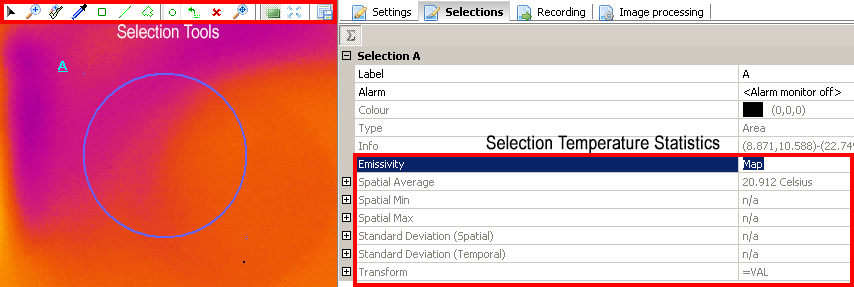
\includegraphics[width=0.7\linewidth]{Figures/3.Chapter/xeneth3.png}
\caption{Xeneth: Selection Panel}
\label{fig:xeneth3}
\end{figure}
\subsubsection{Offset Calibration}
\par When the user selects any of the factory calibrations, there is something that may not seem right. A simple blackbody with constant temperature may appear to have temperature variations as it can be seen in the left of Figure \ref{fig:xeneth5}. This happens due to the Dionisio effect. The Dionisio effect is the reflection of the camera on itself and it is a great error source, so it needs to be eliminated. \\
\begin{figure}[h]
\centering
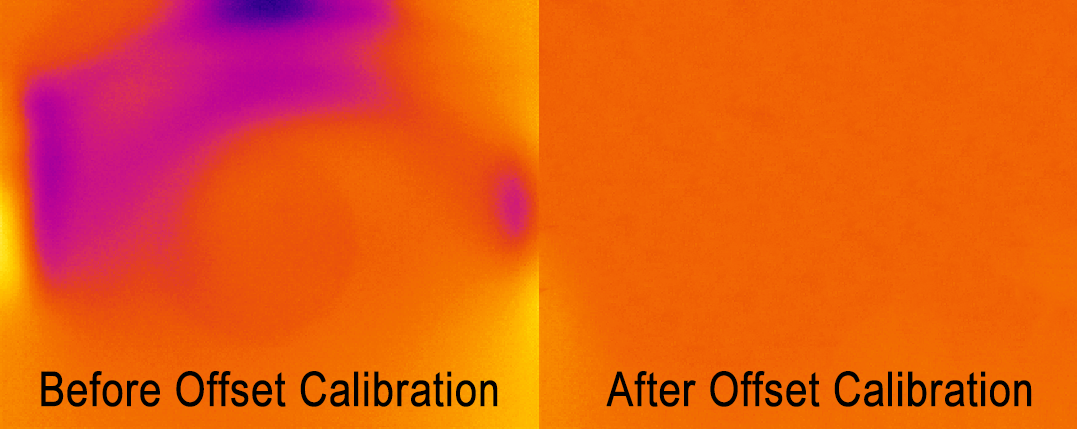
\includegraphics[width=0.7\linewidth]{Figures/3.Chapter/xeneth5.png}
\caption{Offset Calibration: Before and After}
\label{fig:xeneth5}
\end{figure}
\par A good way to eliminate this error is to use a software tool: the Offset Calibration. This can be found in the Calibration Wizard (a menu of calibration options for the camera) and has a simple function. It averages the temperature in space and time and sets every pixel to read that temperature. This eliminates the camera's reflection and also part of the noise and bad pixels. A disadvantage of this method is that it sometimes creates lesser periodic noise, which can be a problem to the measurements. The code behind this function is unknown, so the noise source could not be detected and could only be attenuated later in the post-processing stage. The result of the Offset Calibration can be seen in the right side of Figure \ref{fig:xeneth5}. \\